%
% This is Chapter5 file (chap5.tex)
%
\chapter{Association of Intermittency and Microinstabilities} \label{chap:chap5}

    \section{Overview} \label{sec:ovrvw5}

        As discussed in \Cref{sec:app2}, weakly collisional space plasmas are rarely in local
        thermal equilibrium and often exhibit non-Maxwellian electron and ion velocity distributions
        that lead to the growth of microinstabilities (see \Cref{sec:app2}). These instabilities
        play an active role in the evolution of space plasmas (see \Cref{sec:app2}), as does
        ubiquitous broadband turbulence induced by turbulent structures (see \Cref{sec:inter3b}).
        This \nameCref{chap:chap5} compares linear and non-linear phenomena of a variety of
        2.5-dimensional and 3-dimensional Particle-In-Cell (PIC) simulation for the forward cascade
        of Alfv\'enic turbulence in a collisionless plasma against the same properties of turbulence
        observed by the Magnetospheric Multiscale Mission (MMS) in the terrestrial magnetosheath and
        the Wind spacecraft in the solar wind at 1\,au.

        Both the simulation and the observations show that strong temperature anisotropies and
        growth rates occur highly intermittently in the plasma, and the simulation further shows
        that such anisotropies preferentially occur near current sheets. This suggests that, though
        microinstabilities may affect the plasma globally, they act locally and develop in response
        to extreme temperature anisotropies generated by turbulent structures.

        \Cref{sec:intr5} starts with the introduction of the topic and the motivation for such a
        study. We discuss the data analysis technique in \Cref{sec:danl5} (PIC data in
        \Cref{sec:pic5} and spacecraft data in \Cref{sec:sco5}). \Cref{sec:res5} presents the result
        highlighting the observations made using the different datasets and ends with the conclusion
        and some discussion of further possibilities in \Cref{sec:conc5}.\footnote{Part of this
        study was published in \citet{Qudsi2020a}.}

    \section{Introduction}\label{sec:intr5}

        The focus of this study was protons and in particular their temperature anisotropy\index{anisotropy} ($R_{\rm
        p}$) (see \Cref{eq:aniso}). As discussed in \Cref{sec:instab}, a sufficient departure of
        $R_{\rm p}$ from $R_{\rm p}=1$ triggers one or more modes of \index{microinstability}. These linear
        instabilities and their thresholds are predicted by linear Vlasov theory (see
        \Cref{sec:instab}) under the assumption of a homogeneous background of magnetic field.
        However, the space plasma is rarely homogeneous which raises a fundamental issue of
        reconciling the assumptions of theory of microinstabilites with the observed state of space
        plasma. Multiple studies have shown space plasma to be highly structured and thus
        inhomogeneous \citep{Burlaga1968, Tsurutani1979, Ness2001, Osman2012, Osman2012a,
        Greco2012}. This has been a persistent question in the field and a prime motivation for our
        work which formalizes the implications of \citet{Osman2012}.

        As was highlighted in \Cref{sec:conc2}, owing to inhomogeneous nature of the plasma
        background an ideal study would include the effect of these background inhomogenities in
        computing the growth rates. However we do not have any such established methodology and
        development of such a method is beyond the scope of this study. We thus are restricted to
        use the established theory of microinstabilities, and calculate instability thresholds from
        linear Vlasov equations as discussed in \Cref{sec:intr2}.

    \section{Data and Analysis} \label{sec:danl5}

        \subsection{PIC Simulation}\label{sec:pic5}

            Linear Vlasov calculations were applied to the output of a variety of fully kinetic,
            particle-in-cell (PIC) simulation in homogeneous, collisionless, magnetized plasmas.
            \Cref{tab:datachap} gives detail of different simulation and the starting value of
            important parameters of each data set.

            For 2.5-D simulations, though all vector quantities (like magnetic field $\mathbf{B}$,
            current density $\mathbf{J}$ etc.) had three components they varied only in the
            $xy$-plane for simulation \texttt{149p6} and perpendicular to the $xy$-plane for
            simulation \texttt{kaw} (see \Cref{chap:chap4} for a detailed discussion of different
            types of dataset used in this study). For \texttt{149p6} the initial conditions were
            chosen such that the particle distribution was Maxwellian, $\beta_{\rm p}=\beta_{\rm
            e}=\, 1.2, R_{\rm p}=1, T_{\rm p} = T_{\rm e}$ and the rms value of fluctuations in
            magnetic and velocity fields were half of the background values. For \texttt{kaw} the
            simulation had $\beta_{\rm p}=\beta_{\rm e}=\, 0.6, R_{\rm p}=1, T_{\rm p} = T_{\rm e}$
            as the initial condition whereas for the full 3-D simulation (\texttt{ros}) we had
            $\beta_{\rm p}=\beta_{\rm e}=\, 0.5, R_{\rm p}=1, T_{\rm p} = T_{\rm e}$ and the
            background magnetic field was in $z$-direction. \Cref{tab:datachap} lists out the
            details of all three simulations (and other datasets) in tabular form. It is worth
            noting that high $\beta$-values as well as values much lower than 1 makes the PIC
            computations very expensive and thus were avoided. After the initial condition was
            finalized, the system was allowed to evolve without any external forcing. Fluctuation in
            the observed magnetic and velocity fields produce and drive the turbulence in the
            plasma.

            Once the simulation data was ready, we computed the value of linear growth rates
            ($\gamma_{\max}$) at each point using methodology discussed in \Cref{sec:cgr}. Results
            pertaining to this analysis is discussed in \Cref{sec:picr5}

        \subsection{Space Observations}\label{sec:sco5}

            Similar analysis was carried out on data from two separate space missions: MMS and Wind.
            MMS is a constellation of four identical spacecraft designed to study reconnection in
            the magnetosphere of the Earth \citep{Burch2016}. We used proton density and
            temperature-anisotropy data from the Fast Plasma Investigation (FPI) and magnetic-field
            data from the Fluxgate Magnetometer (FGM). In burst mode FPI measures one proton
            distribution every 150 ms \citep{Pollock2016}, and the cadence of FGM is 128 Hz~
            \citep{Russell2016} (see \Cref{sec:mms} for a more detailed discussion of MMS and some
            of its instruments).

            The measured temperature-anisotropy and magnetic field vectors were used to compute the
            value of the linear instability growth rates ($\gamma_{\max}$) for each point in the
            time series using the same methodology as described in \Cref{sec:intr2}. Though the
            analysis was carried out on several intervals of burst-mode (high cadence) measurements,
            here only results from a 40-minute long period of burst data from 26-12-2017 starting at
            06:12:43 UTC is being presented (see \Cref{tab:mmsdata}). This period was chosen in part
            because of its relatively long duration compared to typical burst mode intervals. During
            this period, average proton density was $22 \,\mathrm{cm}^{-3}$, the average value of
            $\beta_{\parallel \rm p}\, \mathrm{was}$ 4.5 and average bulk velocity of the plasma was
            $238\, \mathrm{km/s}$. \citet{Parashar2018a} describes this data interval in more
            detail.

            For the case of solar wind, we used the data from Wind spacecraft's Faraday Cup (FC) and
            Magnetic Field Investigation (MFI) instruments (see \Cref{sec:wind} for a more detailed
            discussion of instruments and dataset).

    \section{Results} \label{sec:res5}

        \subsection{PIC simulation} \label{sec:picr5}

            \Crefrange{fig:brjhb}{fig:brjros} show five parameters --- $R_{\rm p}$,
            $\beta_{\parallel \rm p}$, $J_{\rm z}$, $\gamma_{\parallel \max}$ and
            $\gamma_{\nparallel \max}$ --- across the simulation box for three different simulations
            (\texttt{149p6}, \texttt{kaw} and \texttt{ros} respectively). For the 3-D case
            (\Cref{fig:brjros}), we show the variation of parameters for a selected slice of
            $xy$-plane.

            Panels (a) to (c) of each (\Crefrange{fig:brjhb}{fig:brjros}) show the three parameters
            --- $R_{\rm p}$, $\beta_{\parallel \rm p}$, and $J_{\rm z}$ --- across the simulation
            box. In all the cases the system is strongly turbulent and exhibits structures of
            various scales. The extreme values of each parameter occur in distinct regions that
            occupy only small fractions of the total volume. That is, these quantities are
            intermittent, which is correlated with the existence of sharp gradients and coherent
            structures \citep{Greco2014, Matthaeus2015, Greco2016, Perrone2016, Perrone2017}.
            Further, extreme values of $R_{\rm p}$ and $\beta_{\parallel \rm p}$ reside near (but
            are not exactly coincident with) extreme values of $J_{\rm z}$. These concentrations of
            current densities frequently correspond to current sheets, as reported by
            \citet{Parashar2016}.

            \begin{figure}
                \begin{center}
                    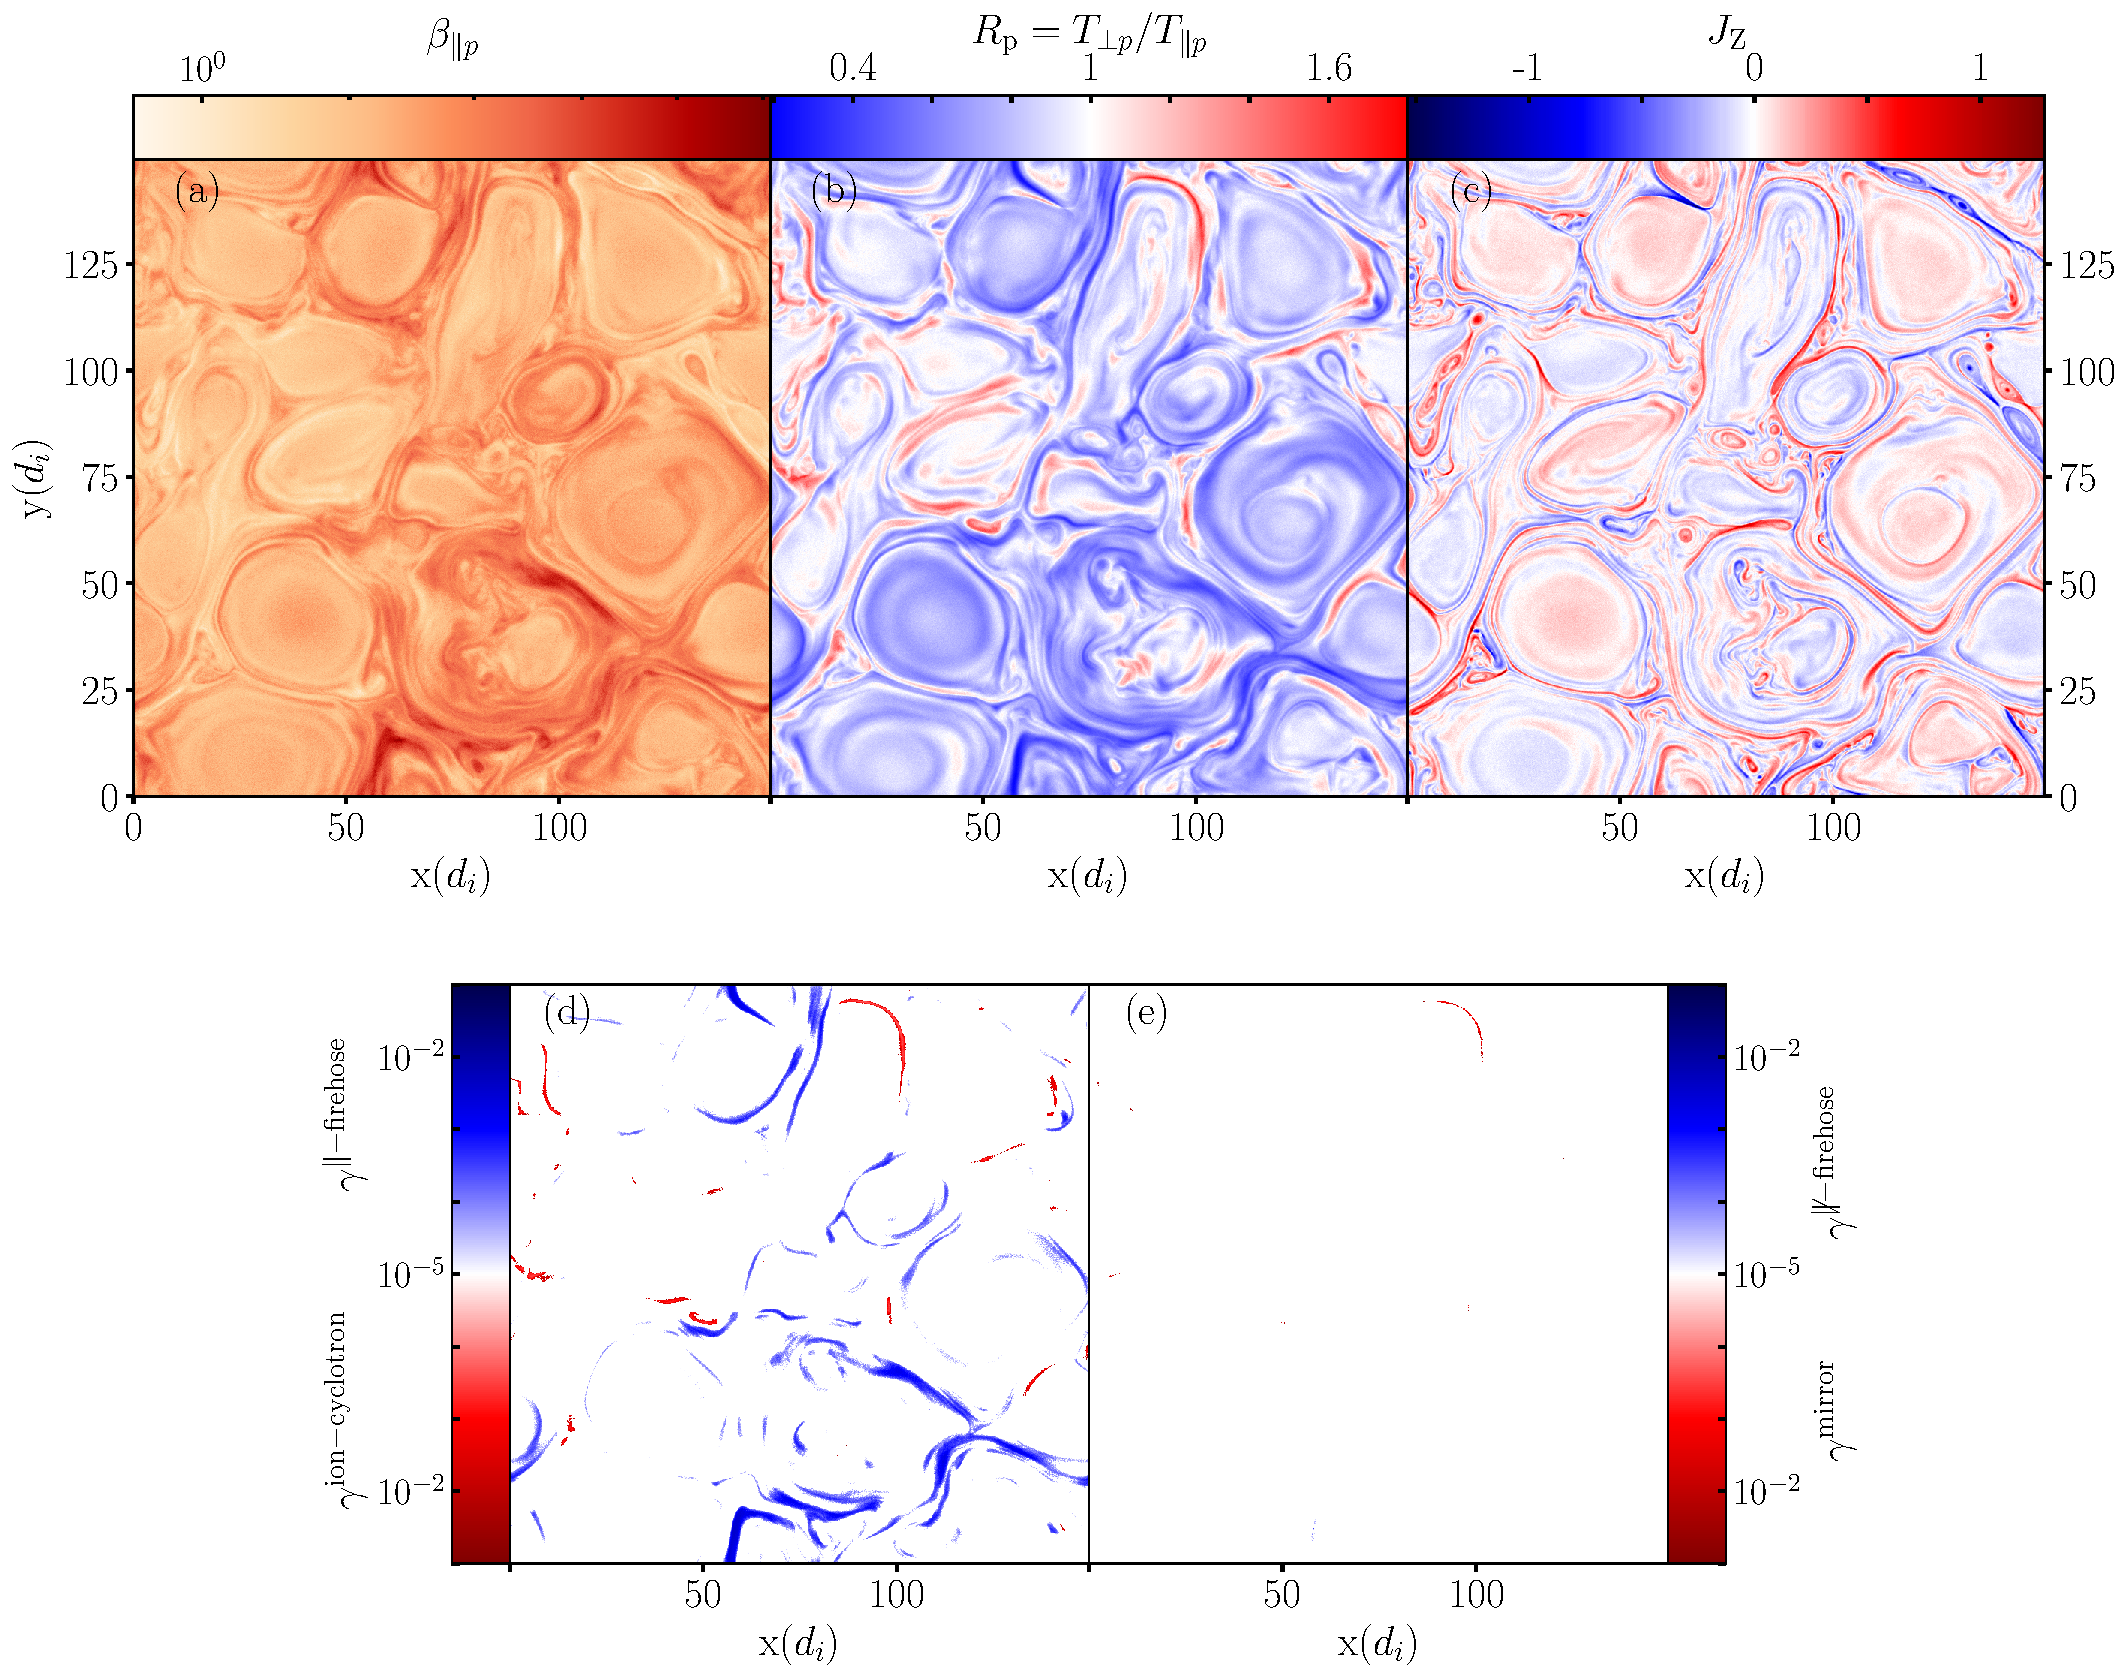
\includegraphics[width=1\textwidth]{figures/chap5/data_Rp_betap_jz_b_149p6_hb_gamma_k_149p6_hb.pdf}
                    \caption[Plot of $\beta_{\parallel \rm p}, R_{\rm p}, J_{\rm z} \mathrm{\,and\,}
                    \gamma$ for \texttt{149p6} dataset]{Colorplot of (top row, left to right)
                    $\beta_{\parallel \rm p}, R_{\rm p} \mathrm{\,and\,} J_{\rm z}$ for
                    \texttt{149p6} dataset. Panel (d) and (e) (bottom row) show the spatial
                    distribution of $\gamma_{\max}$ for parallel and oblique propagation
                    respectively corresponding to first two panels. \textit{Figure reproduced from
                    \citet{Qudsi2020a} with the permission of
                    \href{https://publishing.aip.org/}{AIP Publishing}} (see
                    \Cref{apdx:D}).}
                    \label{fig:brjhb}
                \end{center}
            \end{figure}

            \begin{figure}
                \begin{center}
                    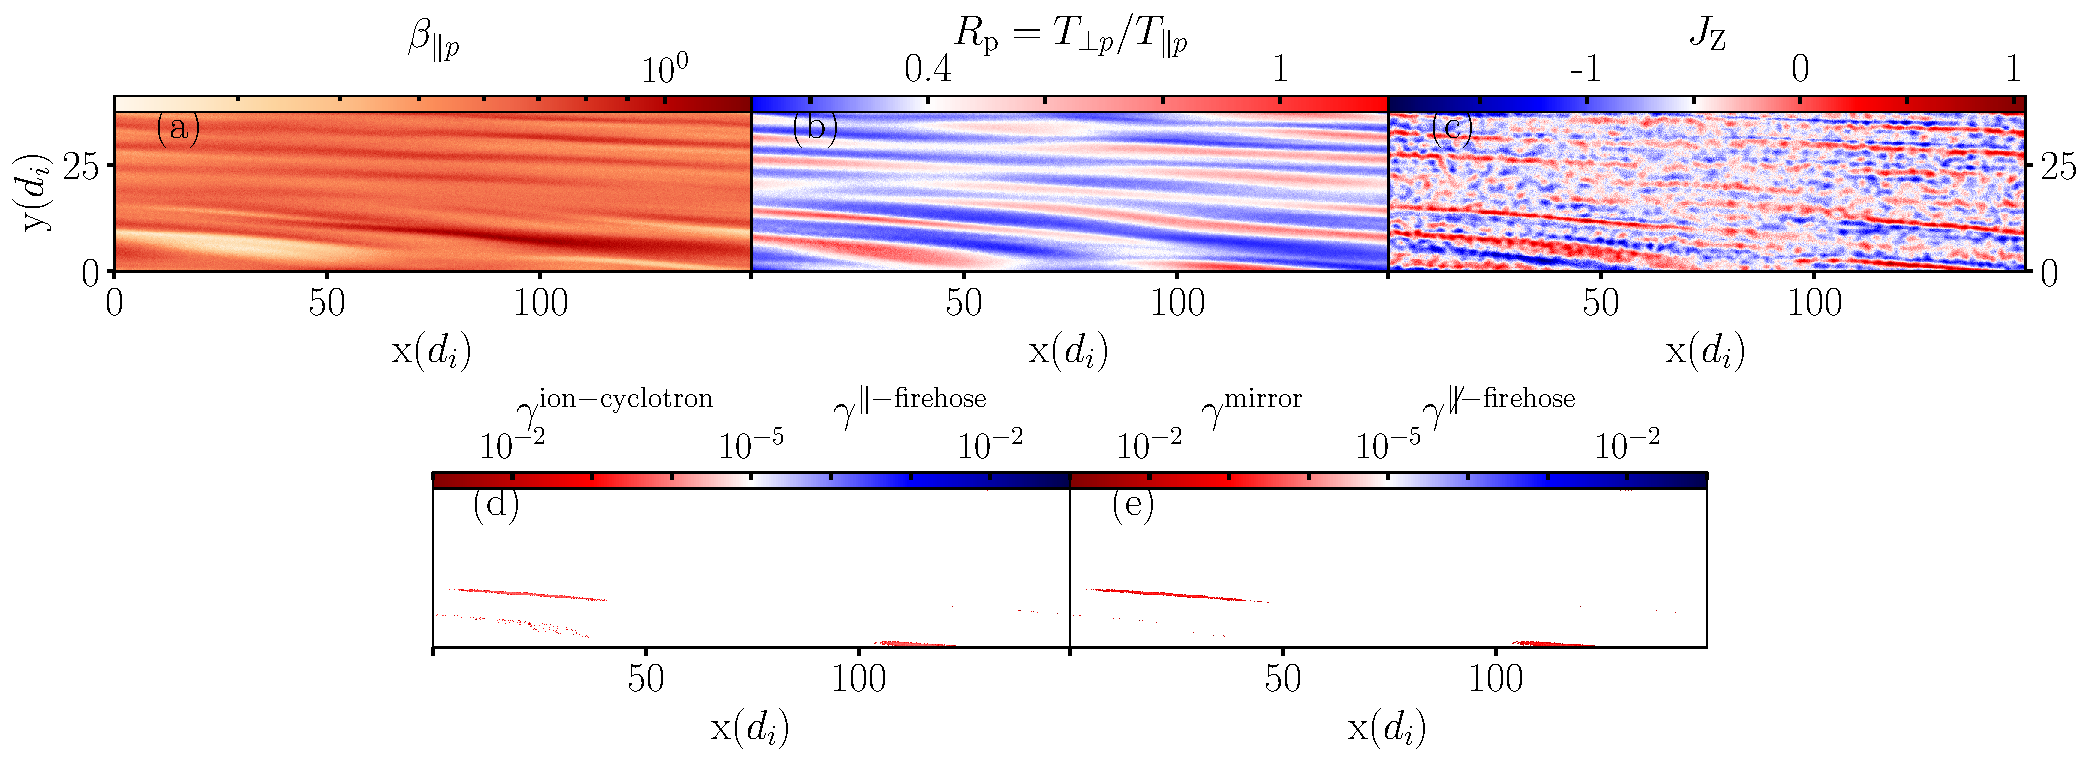
\includegraphics[width=1\textwidth]{figures/chap5/data_Rp_betap_jz_b_kaw_ti0p6te0p6_Time6000wpe_gamma_k_kaw_ti0p6te0p6_Time6000wpe.pdf}
                    \caption[Plot of $\beta_{\parallel \rm p}, R_{\rm p}, J_{\rm z} \mathrm{\,and\,}
                    \gamma$ for \texttt{kaw} dataset]{Colorplot of (top row, left to right)
                    $\beta_{\parallel \rm p}, R_{\rm p} \mathrm{\,and\,} J_{\rm z}$ for \texttt{kaw}
                    dataset. Panel (d) and (e) (bottom row) show the spatial distribution of
                    $\gamma_{\max}$ for parallel and oblique propagation respectively corresponding
                    to first two panels.}
                    \label{fig:brjkaw}
                \end{center}
            \end{figure}

            \begin{figure}
                \begin{center}
                    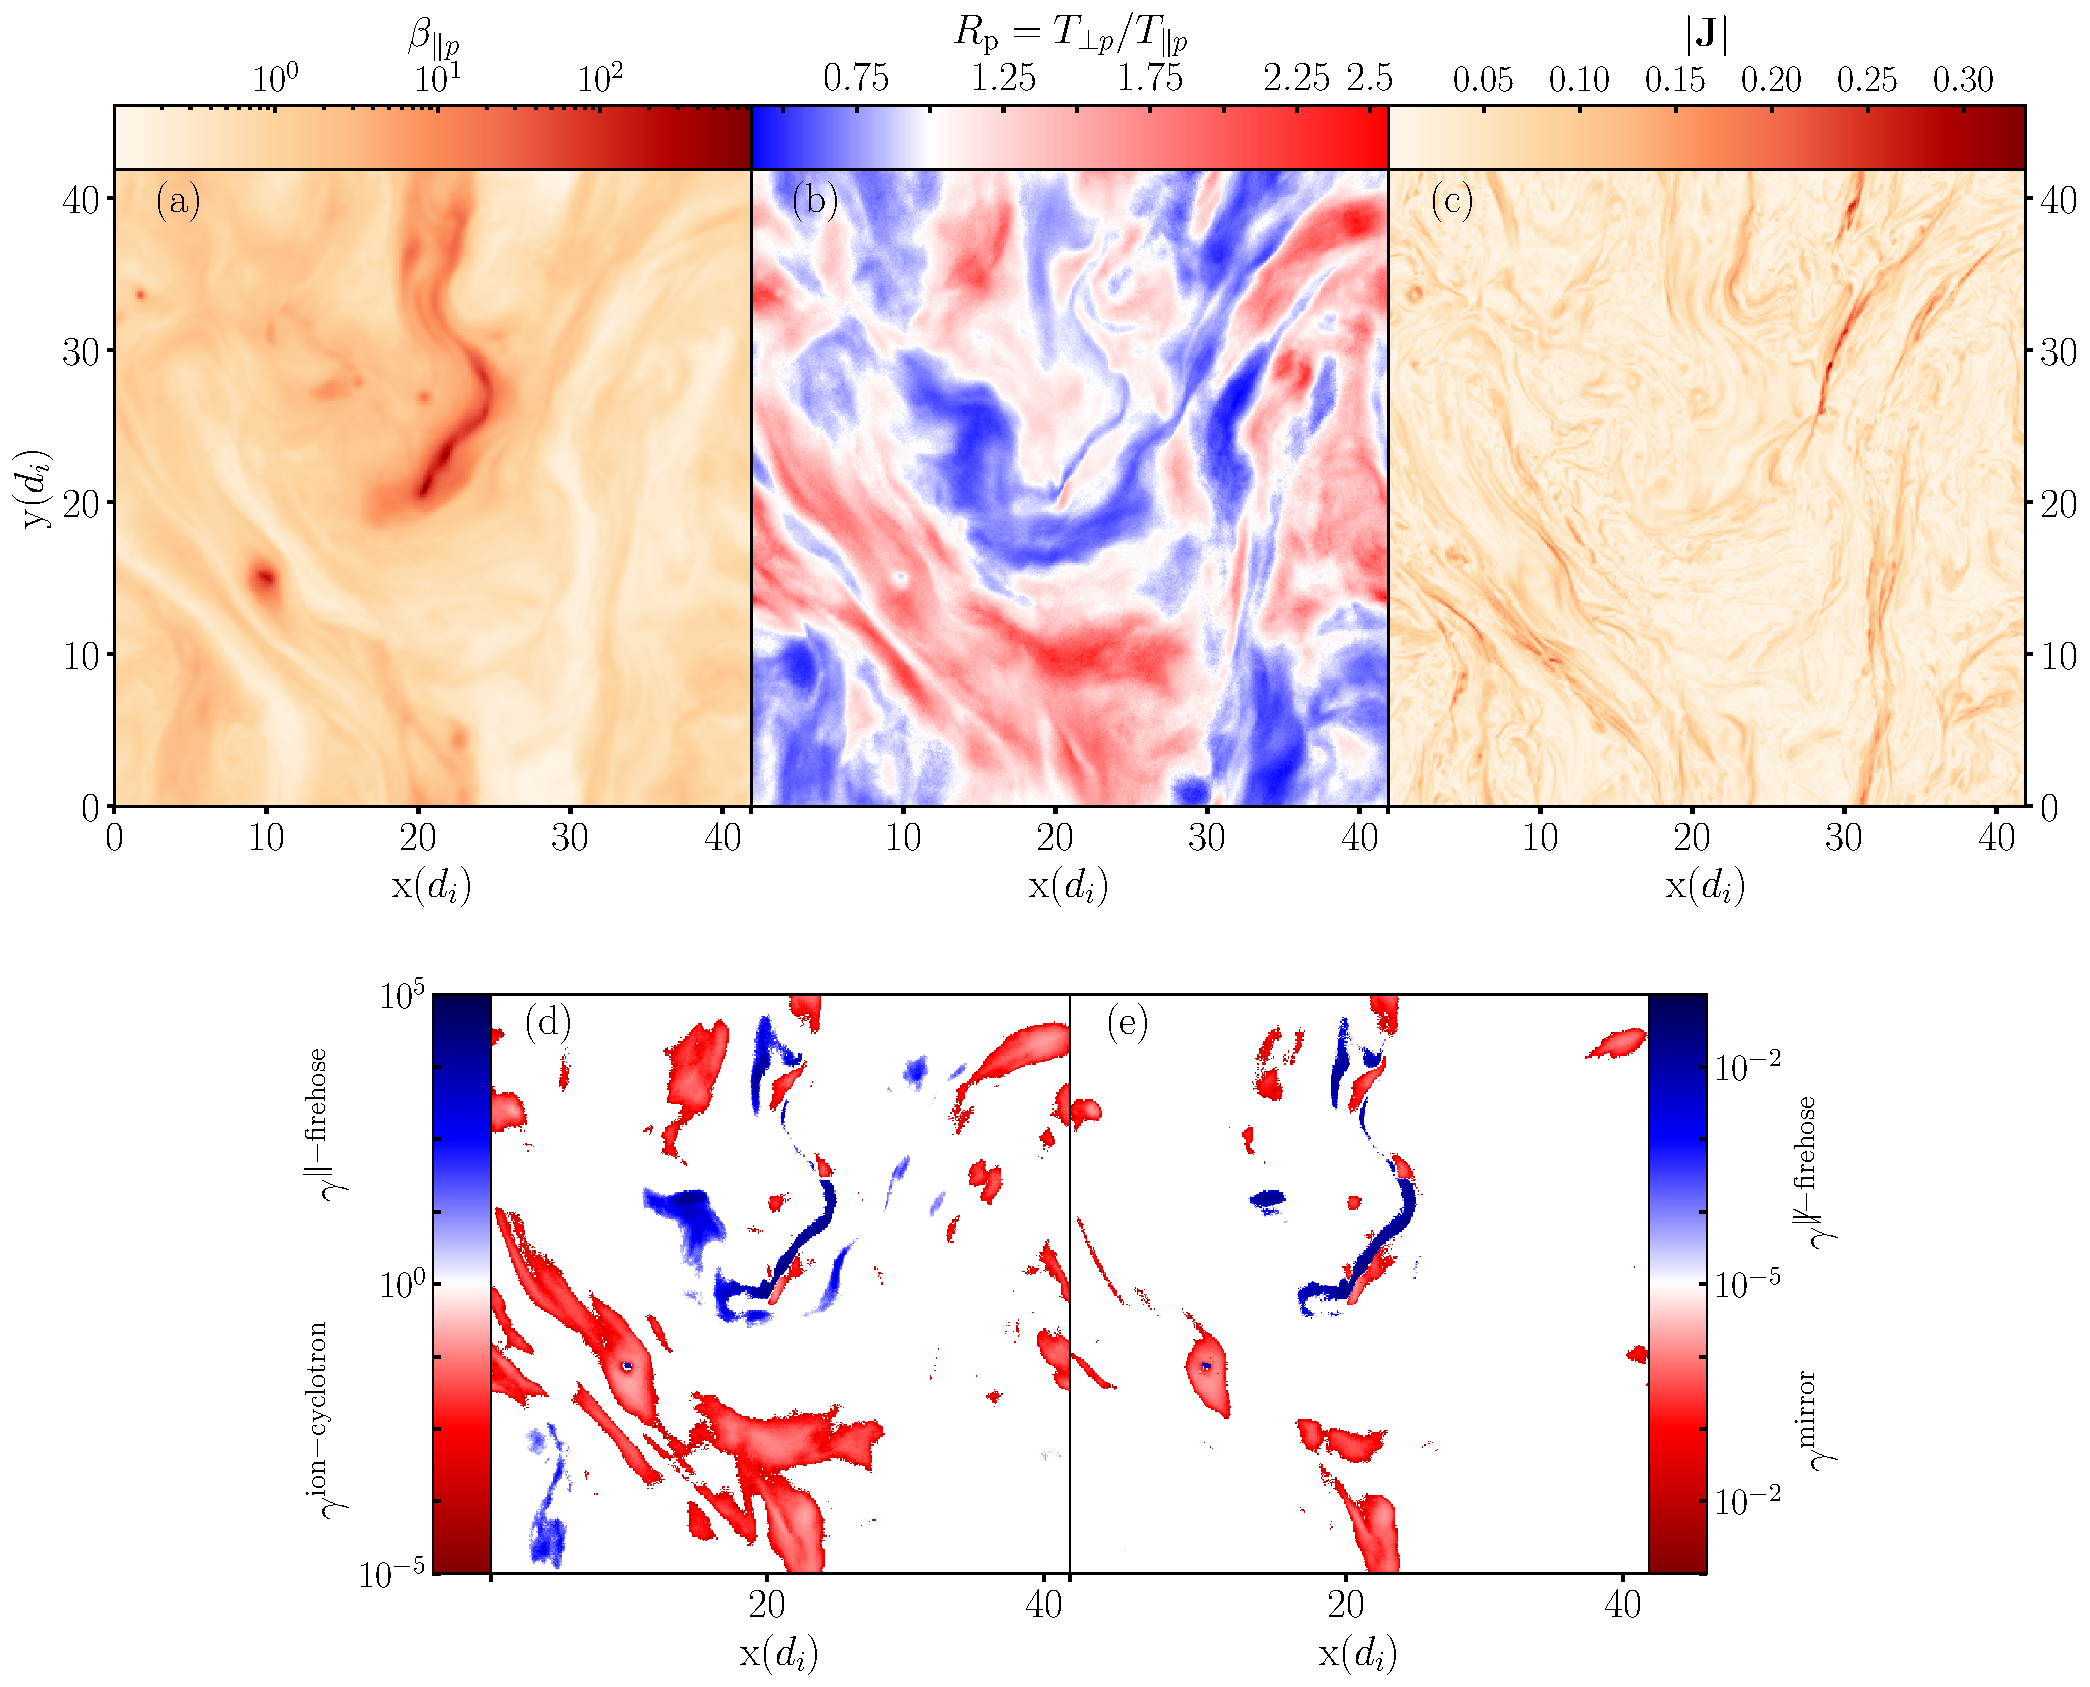
\includegraphics[width=1\textwidth]{figures/chap5/3Ddata_Rp_betap_b_yan512_gamma_k_yan_512.pdf}
                    \caption[Plot of $\beta_{\parallel \rm p}, R_{\rm p}, J_{\rm z} \mathrm{\,and\,}
                    \gamma$ for \texttt{ros} dataset]{Colorplot of (top row, left to right)
                    $\beta_{\parallel \rm p}, R_{\rm p} \mathrm{\,and\,} J_{\rm z}$ for \texttt{ros}
                    dataset. Panel (d) and (e) (bottom row) show the spatial distribution of
                    $\gamma_{\max}$ for parallel and oblique propagation respectively corresponding
                    to first two panels.}
                    \label{fig:brjros}
                \end{center}
            \end{figure}

            Using the method described in \Cref{sec:cgr,chap:chap4}, we computed
            $\gamma_\mathrm{\max}$ for the $(\beta_{\parallel \rm p},R_{\rm p})$-pair at each grid
            point of the simulation box, where $\gamma_\mathrm{\max}$ is the maximum value of growth
            rate for all possible values of propagation vector (\textbf{k}). The fourth and fifth
            Panels (d) and (e) of \Crefrange{fig:brjhb}{fig:brjros} show the spatial distribution of
            growth rates for the solutions with positive growth rates, corresponding to the first
            two panels of the same figure. As described in \Cref{sec:cgr}, for
            $\gamma_\mathrm{max}$, we imposed a cut-off at $10^{-5}\,\Omega_{\rm p}$; thus growth
            rates less than $10^{-5}\,\Omega_{\rm p}$ are considered to be 0. The Panel (d) of each
            figure (\Crefrange{fig:brjhb}{fig:brjros}) corresponds to the parallel modes (cyclotron
            for $R_{\rm p} > \,1$ and parallel firehose for $R_{\rm p} < \,1$), whereas the Panel
            (e) are for the oblique propagation (mirror for $R_{\rm p} > \,1$ and oblique firehose
            for $R_{\rm p} < \,1$). The paucity of blue color in the fifth panel of
            \Cref{fig:brjhb,fig:brjkaw} implies that the $\beta_{\parallel \rm p}$ (and/or $R_{\rm
            p}$) was rarely high (low) enough to excite any mode of oblique firehose instability.

            Comparing Panel (b) to Panel (d) and (e) of these figures, we see that values of
            $\gamma_\mathrm{max}>0$ are concentrated in distinct, thin regions of the $xy$-plane
            where extreme values of temperature anisotropy also occur. We also note that, for
            \Cref{fig:brjhb} because the simulation is 2.5D with $\mathbf{B_{\rm 0}}$ perpendicular
            to the simulation plane, the growth of instabilities such as the proton cyclotron and
            the parallel proton firehose with maximum growth at $\mathbf{k \times B_{\rm 0} = 0}$ is
            suppressed. However, for the other two simulations (\Cref{fig:brjkaw,fig:brjros}) that
            is not the case. Consequently, we see a lot of parallel instability in \Cref{fig:brjros}
            and a much higher value of average growth rate for \texttt{kaw} and \texttt{ros}
            datasets compared to \texttt{149p6} (see \Cref{fig:ratio_kde_all} and associated
            discussion). However, despite not being suppressed in the parallel direction, parallel
            instabilities in \Cref{fig:brjkaw} remain relatively sparse because of very low value of
            $\beta_{\parallel \rm p}$ (see \Cref{tab:datadetail4a}). Comparatively \Cref{fig:brjros}
            shows much less sparsity as a consequence of high value of $R_{\rm p}$ over an extended
            region of the simulation box.

        \subsection{Spacecraft Observations} \label{sec:spcr5}

            \begin{sidewaysfigure}
                \begin{center}
                    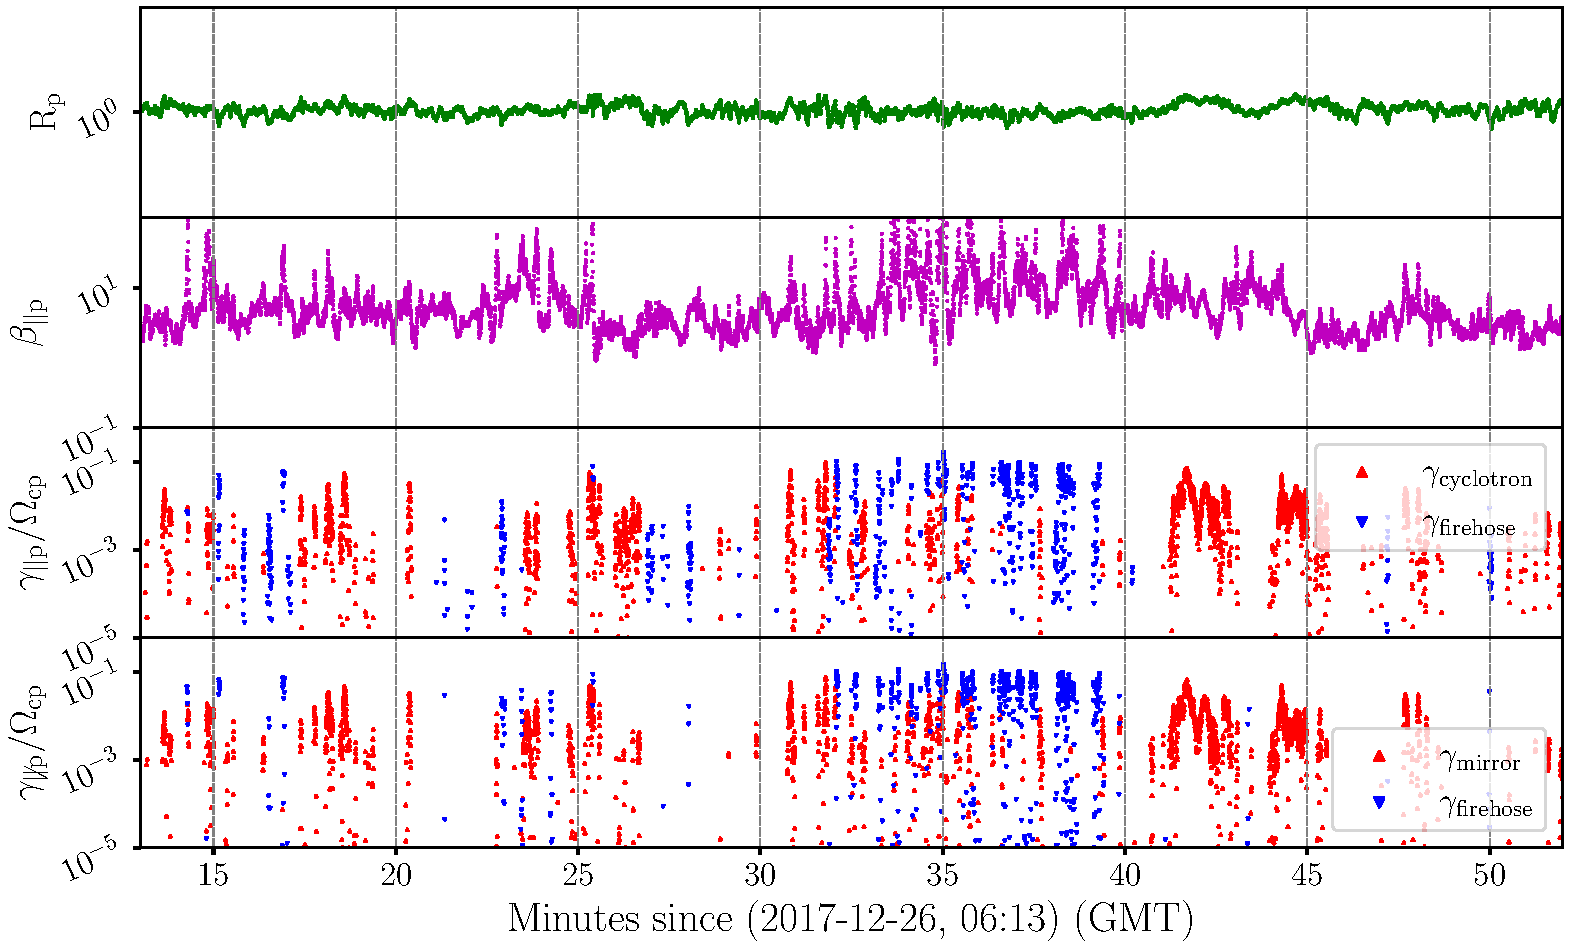
\includegraphics[width=1.\textwidth]{figures/chap5/mms_all_piecewise_2017-12-26_2017-12-26_00000108_00015707.pdf}
                    \caption[Time series plot of $\beta_{\parallel \rm p}, R_{\rm p}, J_z
                             \mathrm{\,and\,} \gamma$ for \texttt{mms} dataset]{Time series plot of
                             proton anisotropy ratio $(R_{\rm p})$, proton parallel beta
                             $(\beta_{\parallel \rm p})$, total current density in
                             $\mathrm{nA/m^2}$, parallel instability growth rates (proton-cyclotron,
                             in red and parallel firehose in blue), and oblique instability growth
                             rates (mirror in red and oblique firehose in blue), as observed by MMS
                             on 2017 December 26.}
                    \label{fig:brjmms}
                \end{center}
            \end{sidewaysfigure}

            \begin{sidewaysfigure}
                \begin{center}
                    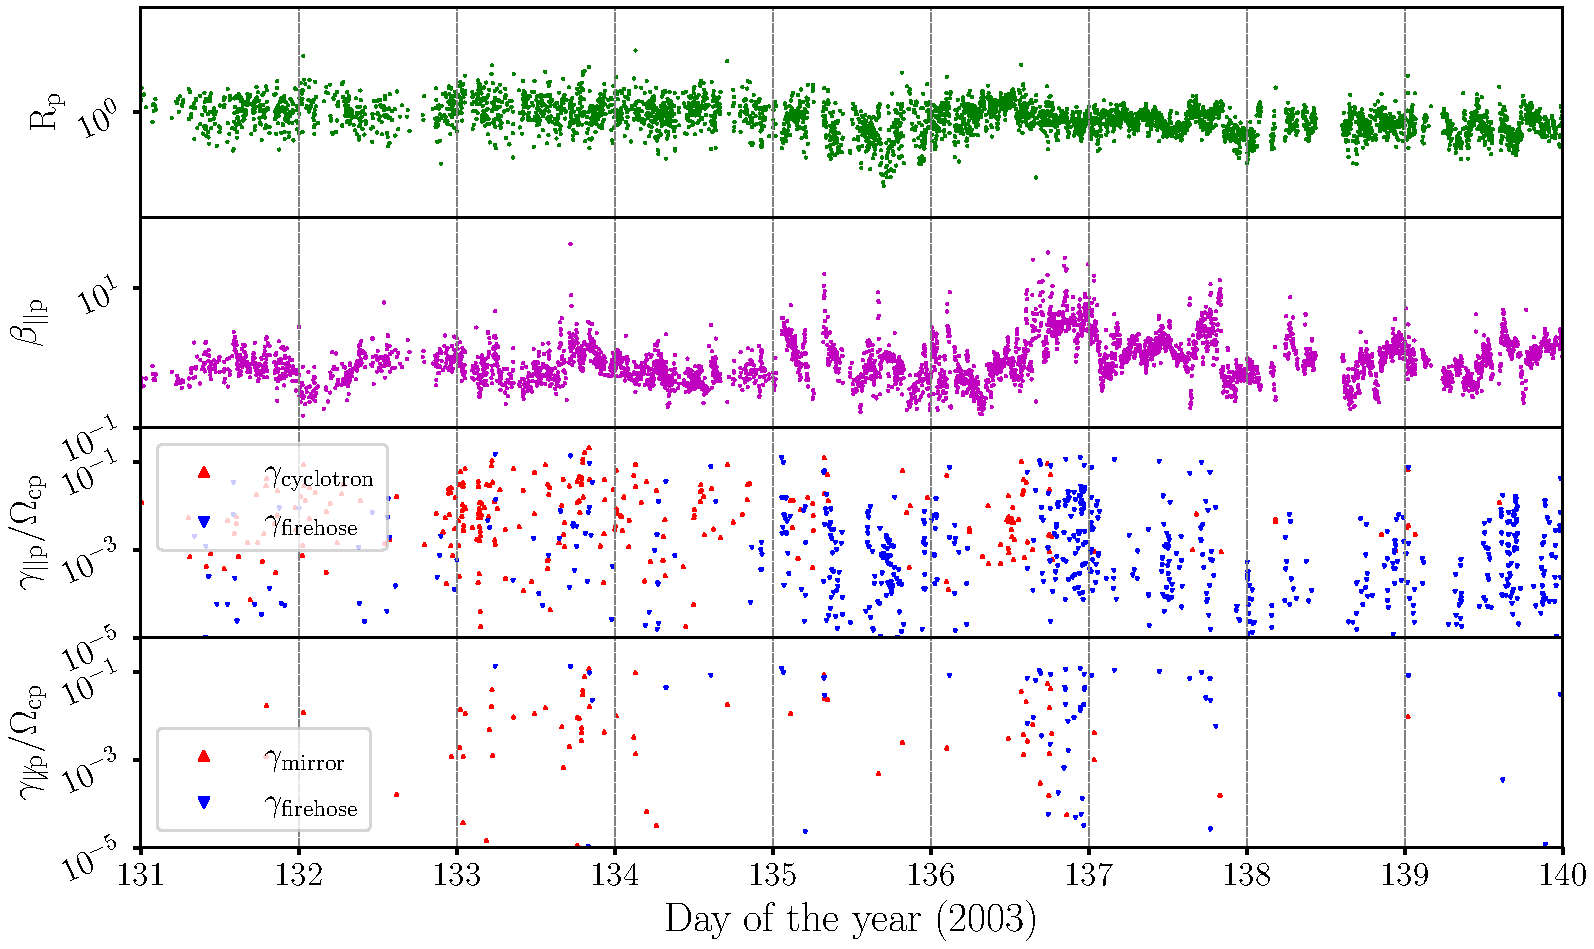
\includegraphics[width=1.\textwidth]{figures/chap5/wind_all_piecewise_2003-5-11_2003-5-19_01207878_01212368.pdf}
                    \caption[Time series plot of $\beta_{\parallel \rm p}, R_{\rm p}, J_{\rm z}
                             \mathrm{\,and\,} \gamma$ for \texttt{wnd} dataset]{Time series plot of
                             proton anisotropy ratio $(R_{\rm p})$, proton parallel beta
                             $(\beta_{\parallel \rm p})$, parallel instability growth rates
                             (proton-cyclotron, in red and parallel firehose in blue), and oblique
                             instability growth rates (mirror in red and oblique firehose in blue),
                             as observed by Wind.}
                    \label{fig:brjwnd}
                \end{center}
            \end{sidewaysfigure}

            \begin{figure}
                \begin{center}
                    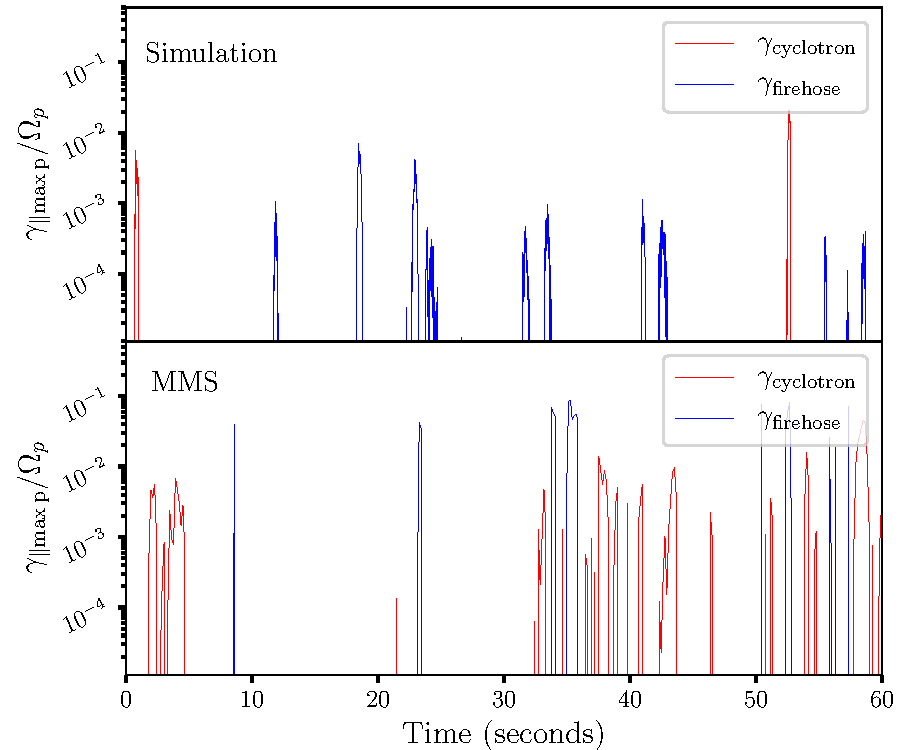
\includegraphics[width=1.\textwidth]{figures/chap5/SpaceCraft_simulation_mms.pdf}
                    \caption[Spacecraft and simulation comparison of $\gamma$ time
                            series]{Comparison of simulation and MMS time series for
                            $\gamma_{\parallel max}$ values for a 1-minute period. The top panel
                            shows the distribution for a 1-minute long flight through the simulation
                            box and the lower panel shows the distribution of $\gamma_\mathrm{max}$
                            starting at 06:34 on 2017 December 26. \textit{Figure reproduced from
                            \citet{Qudsi2020a} with the permission of
                            \href{https://publishing.aip.org/}{AIP Publishing}} (see
                            \Cref{apdx:D}).}
                    \label{fig:spcsim}
                \end{center}
            \end{figure}

            \Cref{fig:brjmms} and \Cref{fig:brjwnd} show a typical portion of the time series data
            from two spacecraft: MMS and Wind. The panels, from top to bottom show $R_{\rm p},
            \beta_{\parallel \rm p}, |\mathbf{J}|$ and maximum growth rates ($\gamma_\mathrm{max}$)
            for parallel and oblique instabilities respectively for both the spacecraft. Time
            intervals were chosen so that the figures showed approximately equal numbers of
            correlation time scales in the magnetosheath and solar wind at 1\,au. For magnetosheath
            10 minute corresponds to roughly 20 $\tau_{\rm cr}$ \citep{Le1993,Gutynska2008} whereas
            for solar wind which has a correlation time length of about 55 minutes the interval of
            24 hours corresponds to about 25 times $\tau_{\rm cr}$ \citep{Matthaeus1982,Wicks2010}.

            Both the \Cref{fig:brjmms,fig:brjwnd} show an intermittent distribution of instability
            growth rates, though in case of Wind since the variation in $\beta_{\parallel \rm p}$ is
            much smaller than that observed in magnetosheath the number of unstable points are
            significantly smaller. \Cref{tab:datadetail4a} lists out the variation in these
            parameters for all the different cases discussed so far.

            \begin{table}[ht]
                \centering
                \caption[Average value of parameters for datasets]{Average values of parameters for
                different datasets}
                \begin{tabular}{ p{0.1\linewidth} p{0.30\linewidth} p{0.1\linewidth}
                p{0.1\linewidth} p{0.12\linewidth}}
                    \hline
                    \\
                    Name & Type of data & $\left<\beta_{\parallel \rm p}\right>$ & $\left<R_{\rm
                    p}\right>$ & $n_\gamma/N$ (\%)\\
                    \\
                    \hline
                    \\
                    \texttt{149p6} & Simulation & 0.64 & 0.83 & 6.82 \\
                    \\
                    \hline
                    \\
                    \texttt{kaw} & Simulation & 0.61 & 0.89 & 0.90 \\
                    \\
                    \hline
                    \\
                    \texttt{ros} & Simulation & 0.84 & 1.04 & 16.39 \\
                    \\
                    \hline
                    \\
                    \texttt{mms} & Spacecraft \newline Observation\newline (Magnetosheath) & 4.29 &
                    1.04 & 24.51 \\
                    \\
                    \hline
                    \\
                    \texttt{wnd} & Spacecraft \newline Observation\newline (Solar Wind) & 0.69 &
                    0.50 & 14.22 \\
                    \\
                    \hline
                \end{tabular}
                \label{tab:datadetail4a}
            \end{table}

            Comparing \Cref{fig:brjhb} and \Cref{fig:brjmms} we see that a larger fraction the MMS
            data ($30\%$) are unstable versus grid points from the simulation ($0.8\%$), with
            $\gamma_\mathrm{max}$ values above the cut-off ($10^{-5}\,\Omega_{\rm p}$). This
            discrepancy arises in part because MMS data have much higher values of $\beta_{\parallel
            \rm p}$ than the simulation (median values of 4.5 and 1.2, respectively). Furthermore,
            \citet{Servidio2015} found that, for a given value of $\beta_{\parallel \rm p}$,
            simulations of the turbulence type, like in the present 2.5D cases, generally admit less
            extreme temperature-anisotropy than are seen in space observations, because typical
            simulations are of modest size resulting in modest Reynolds number and lack large scale
            coherent driving.

            The time series for MMS observation (\Cref{fig:brjmms}) exhibits intermittent structure
            in the distribution of growth rates that are similar to what we see in Panels (d) and
            (e) of \Cref{fig:brjhb} for simulation. \Cref{fig:spcsim}, which shows the comparison of
            the time series of simulation and MMS data for a 1\,minute period, shows that
            qualitatively they have similar distribution. Time series for the simulation was
            computed by flying a virtual spacecraft, travelling at the plasma bulk speed (238\,km/s,
            same speed as that of plasma during MMS observation), through the entire box at an angle
            of 75 degrees with respect to $x$-direction.

            In \Cref{fig:brjmms} the points of instabilities ($\gamma_\mathrm{max}>0$) are
            concentrated together, spreading over a small time interval lasting typically a few
            seconds (4-8\,seconds) with sharp peaks. Though in this study we did not quantify the
            length scale of all the peaks, we found that typically they are spread over a length
            scale of $\sim 20-40\,\mathrm{d_{\rm i}}$, where $\mathrm{d_{\rm i}}$ is the
            ion-inertial length and the length scale was calculated using the flow speed of the
            plasma and the duration of the peak.

    \section{Discussions} \label{sec:conc5}

        In recent years, two different perspectives have been widely used to explain the behavior of
        the solar wind, magnetosheath, and similar space plasmas. In the first picture, the linear
        theory of plasma instability, at high $\beta_{\parallel \rm p}$, for extreme $R_{\rm p}$,
        different instability thresholds become active, thereby confining the plasma population to
        lower values of $R_{\rm p}$
        \citep{Gary2001,Kasper2002,Hellinger2006,Matteini2007,Klein2018}. In the second, turbulence
        generates sharp gradients in the plasma that produce temperature anisotropy
        \citep{Osman2011,Greco2012,Valentini2014,Parashar2016}.

        These two theories have been non-reconcilable because of the basic underlying assumption.
        The linear theory of plasma instability assumes a homogeneous background magnetic field
        whereas turbulence relies on large fluctuations in the field. It was hitherto unclear if
        these two seemingly disparate processes--microinstabilities and turbulence\index{turbulence}--are connected in
        any way in configuration space. The apparent contradiction---homogeneity against
        intermittent inhomogeneity---between the two interpretations poses a question of fundamental
        importance in the study of space plasmas specifically and collisionless plasmas in general:
        How can an inhomogeneous phenomenon such as turbulence be consistent with
        temperature-anisotropy constraints derived from linear theory of homogeneous plasmas? Our
        simulations show that the turbulence indeed heats the plasma anisotropically, making it more
        susceptible to instability. But the simulation also show that these anisotropies are
        strongly localized; furthermore the 2.5-D character of the simulation with a strong
        background magnetic field out of the simulation plane acts against the growth of the proton
        cyclotron and parallel proton firehose microinstabilities. Clearly, further studies are
        necessary to resolve this apparent contradiction.

        Although there is no discussion of the consequences of electron anisotropies here, it should
        be noted that both simulations and magnetosheath observations \citep{Gary2005} have shown
        that electron temperature anisotropies in collisionless plasmas can drive whistler
        instabilities which, in turn, scatter the electrons to establish a constraint on the
        anisotropy of that species \citep{Gary1996}, in full analogy with the case of ion
        instabilities and anisotropy constraints discussed here.

        In \Crefrange{fig:brjhb}{fig:brjros} the regions of significant growth rates are close to
        the regions of peak current values. This suggests that current sheets are producing the
        extreme temperature-ansiotropies that ultimately drive the instabilities. Note, though, that
        the high-$\gamma_{\max}$ regions and the high-$J_{\rm z}$ regions do not perfectly overlap:
        they tend to be adjacent to each other rather than co-located, as seen by \citet{Greco2012}.
        Thus, traditional methods of correlation calculation would be inadequate to quantify the
        relationship between these two structures. Instead, an analysis using cross correlations of
        these quantities \citep[see, e.g.,][]{Parashar2016} or joint distributions \citep[see,
        e.g.,][]{Yang2017} to explore the causal connection between instabilities and
        turbulence-generated current sheets would be the next step forward.

        In this study we found an explicit connection between intermittency in plasma turbulence and
        indication of the local enhancement of linear instability growth rates. Intermittency is
        clearly influential in the interpretation of observations, while its theoretical importance
        derives from its potential connection to the nature and statistics of dissipation
        \citet{Kolmogorov1962, Karimabadi2013, Wan2016, Howes2015, Matthaeus2015}. The connection we
        have found here---that linear instability growth rates computed from (admittedly
        oversimplified) homogeneous plasma theory, also occur in intermittent bursts---adds to this
        emerging understanding of plasma dissipation. Previous studies found that pathways, such as
        inertial range transfer \citep{SorrisoValvo2019}, electromagnetic work \citep{Wan2012},
        electron energization \citep{Karimabadi2013}, and pressure-strain interactions
        \citep{Yang2017} concentrate in small sub-volumes of plasma turbulence. Dynamical processes
        that lead to dissipation such as magnetic reconnection, also occur in spatially localized
        regions \citep{Drake2008}. Along with these we now have observed strong indication that
        velocity-space driven phenomena \citep{Servidio2012a, Greco2012, Schekochihin2016,
        Servidio2015} also occur in similar highly localized sub-volumes. Observation and study of
        wave signatures which propagate in both directions and thus implying proximity to the
        generation region may provide a more conclusive evidence. The nature of the spatial or
        regional correlations of these kinetic processes to the surrounding dynamical processes that
        drive them largely remains to be explored.